% ------------------------------ %
%                                %
%    Preamble by Rasmus Wiuff    %
%        rwiuff@gmail.com        %
%                                %
% -------------------------------%

%Author(s), Course variables
\newcommand{\titl}{Implementering \& Test}
\newcommand{\handin}{Indsæt dato}
\newcommand{\authOne}{Rasmus Wiuff}
\newcommand{\authTwo}{Mathies Henriksen}
\newcommand{\authThree}{Max-Emil Scotten}
\newcommand{\authFour}{Kasper Sylvest}
\newcommand{\SIDOne}{s163977}
\newcommand{\SIDTwo}{s200747}
\newcommand{\SIDThree}{s204633}
\newcommand{\SIDFour}{s205281}
\newcommand{\courseno}{02161}
\newcommand{\course}{Software Engineering 1}
\newcommand{\lb}{\\}
%Basics
\documentclass[a4paper, danish]{article}
\usepackage[utf8]{inputenc}
\usepackage[T1]{fontenc}
\usepackage[bitstream-charter]{mathdesign}
\usepackage{babel}
\usepackage[moderate]{savetrees}
%Symbols and scientifics
\usepackage{amsmath, bm}
\numberwithin{equation}{section}
\usepackage{physics}
\usepackage{mathtools}
\usepackage{siunitx}
\sisetup{
per-mode = power ,
round-mode = figures ,
round-precision = 3 ,
exponent-mode = input ,
output-decimal-marker = {.} ,
exponent-product = 	imes ,
uncertainty-mode = separate ,
range-phrase = - ,
range-units =  single ,
inter-unit-product = \ensuremath{{\cdot{}}} ,
quantity-product = \ ,
separate-uncertainty-units = single ,
}

%Appendix, TOC and Bibliography
\usepackage{appendix}
\renewcommand\appendixtocname{Appendiks}
\renewcommand\appendixpagename{Appendiks}
\usepackage[nottoc]{tocbibind}
\setcounter{tocdepth}{2}
\usepackage{lastpage}

%Figures
\usepackage[svgnames]{xcolor} % Required to specify font color
\usepackage{float}
\usepackage{graphicx}
\usepackage{subcaption}
\usepackage[format=plain,
    labelfont={bf,it,footnotesize},
    textfont={it,footnotesize}]{caption}
% \captionsetup[table]{name=Huskeord}
\captionsetup{font={stretch=0.9}}
\usepackage{wrapfig}
\usepackage[a4paper, centering, rmargin=2.5cm, tmargin=2.5cm, lmargin=2.5cm, bmargin=3.5cm]{geometry}
\usepackage{verbatim}
\usepackage[space]{grffile}
\usepackage[final]{pdfpages}
\usepackage{pdflscape}
\usepackage{multirow}
\usepackage{fontawesome}
\usepackage{tikz}
\usetikzlibrary{positioning}
\newcommand{\ttt}[1]{\texttt{#1}}
\newcommand{\F}{\mathtt{F}}
\newcommand{\T}{\mathtt{T}}

\newcommand{\lorf}{\ensuremath{\lor\F}}
\newcommand{\lort}{\ensuremath{\lor\T}}
\newcommand{\landf}{\ensuremath{\land\F}}
\newcommand{\landt}{\ensuremath{\land\T}}
\newcommand{\tof}{\ensuremath{\to\!\F}}
\newcommand{\tot}{\ensuremath{\to\!\T}}
\newcommand{\lrf}{\ensuremath{\leftrightarrow\!\F}}
\newcommand{\lrt}{\ensuremath{\leftrightarrow\!\T}}
\newcommand{\negf}{\ensuremath{\neg\F}}
\newcommand{\negt}{\ensuremath{\neg\T}}
\newcommand{\allf}{\ensuremath{\forall\F}}
\newcommand{\allt}{\ensuremath{\forall\T}}
\newcommand{\exf}{\ensuremath{\exists\F}}
\newcommand{\ext}{\ensuremath{\exists\T}}

\newcommand{\first}[2]{\node (root) {\textcolor{red}{\scriptsize 1} \(#1\) : \texttt{#2}};}
\newcommand{\formula}[4]{\node (#1) [#2] {\textcolor{red}{\scriptsize #1} \(#3\) : \texttt{#4}};}
\newcommand{\branch}[2]{\path (#1) edge[-] (#2);}
\newcommand{\rbranch}[4]{\path (#3) edge[-] node [midway, right, blue] {\(#1\) på \(#2\)} (#4);}
\newcommand{\closed}[2]{\node (#1) [below = .1em of #2] {\(\times\)};}
\newcommand{\open}[2]{\node (#1) [below = .1em of #2] {\(\bigcirc\)};}
\newenvironment{tableau}{\begin{tikzpicture}[node distance = .5pt]}{\end{tikzpicture}}

%Header footer
\usepackage{fancyhdr}
\pagestyle{fancy}
\lhead{\titl \lb Kursus \courseno\ \lb \course \lb \handin}
\chead{
\includegraphics[height=40pt]{Graphics/DTU}}
\rhead{\authOne \ \textbf{\SIDOne} \lb \authTwo \ \textbf{\SIDTwo} \lb \authThree \ \textbf{\SIDThree} \lb \authFour \ \textbf{\SIDFour}}
\cfoot{Side \thepage\, af \pageref*{LastPage}}
\renewcommand{\headrulewidth}{0.4pt}
\renewcommand{\footrulewidth}{0.4pt}
\setlength{\headheight}{46.80968pt}
\addtolength{\topmargin}{-10.05934pt}

%Text tools
\usepackage{listings}
\usepackage{parcolumns}
\usepackage[super]{nth}
\usepackage[normalem]{ulem}
\usepackage{import}
\usepackage{url}
\usepackage{lipsum}
\usepackage{microtype}
%\usepackage[draft]{microtype}
\usepackage[pdfencoding=auto, psdextra]{hyperref}
\hypersetup{
    colorlinks   = true, %Colours links instead of ugly boxes
    urlcolor     = blue, %Colour for external hyperlinks
    linkcolor    = blue, %Colour of internal links
    citecolor   = red %Colour of citations
}
\usepackage[capitalise]{cleveref}
% \crefname{table}{Huskeord}{Huskeord}
\usepackage{enumitem}
\newlist{arrowlist}{itemize}{1}
\setlist[arrowlist]{label={\(\rightarrow\)}}
\usepackage{tabularray}
\UseTblrLibrary{booktabs}
\usepackage{todonotes}
\usepackage[square, longnamesfirst, numbers]{natbib}
\usepackage{empheq}
\usepackage[newfloat, outputdir=../]{minted} % Overleaf minted buildpath fix
% \usepackage[newfloat]{minted}
\setminted{fontsize=\small,
           linenos=true}
\usemintedstyle{tango}
\SetupFloatingEnvironment{listing}{listname=Listings}
\newcommand{\im}[3]{\inputminted[linenos=true, python3=true, firstline=#2, lastline=#3]{python}{#1}}
\newcommand{\java}[3]{\inputminted[linenos=true, firstline=#2, lastline=#3]{java}{#1}}
\usepackage{dirtree}

%Definitions and new commands
\newcommand{\degr}{^{\circ}}
\newcommand{\me}{\mathrm{e}}

%Title and sectioning
\def\Vhrulefill{\leavevmode\leaders\hrule height 0.7ex depth \dimexpr0.4pt-0.7ex\hfill\kern0pt}
\usepackage{titlesec}
\usepackage{titling}
\definecolor{DTUred}{cmyk}{0, .91, .72, .23}
\definecolor{FMNgrey}{cmyk}{.73,.43,.53,.38}
%Use letters insted of numbers in section numbering
% \renewcommand{\thesection}{\Alph{section}}
% \renewcommand{\thesubsection}{\Alph{subsection}}

\makeatletter
\newcommand{\github}[1]{%
   \href{#1}{\color{DTUred}\faGithub}%
}
\makeatother

%Algorithms and pseudocode
\newcounter{nalg}[section] % defines algorithm counter for chapter-level
\renewcommand{\thenalg}{\thesection .\arabic{nalg}} %defines appearance of the algorithm counter
\DeclareCaptionLabelFormat{algocaption}{Algoritme \thenalg} % defines a new caption label as Algorithm x.y

\lstnewenvironment{algorithm}[1][] %defines the algorithm listing environment
{
    \refstepcounter{nalg} %increments algorithm number
    \captionsetup{labelformat=algocaption,labelsep=colon} %defines the caption setup for: it ises label format as the declared caption label above and makes label and caption text to be separated by a ':'
    \lstset{ %this is the stype
        mathescape=true,
        frame=tB,
        numbers=left,
        numberstyle=\tiny,
        basicstyle=\scriptsize,
        keywordstyle=\color{black}\bfseries\em,
        keywords={,input, output, return, datatype, function, in, if, else, foreach, for, while, begin, end,} %add the keywords you want, or load a language as Rubens explains in his comment above.
        numbers=left,
        xleftmargin=.04\textwidth,
        #1 % this is to add specific settings to an usage of this environment (for instnce, the caption and referable label)
    }
}
{}

\begin{document}

\titleformat{\section}[block]
{\normalfont\Large\scshape\filright\color{DTUred}}{\fbox{\thesection}}{1em}{}

\titleformat{\subsection}
{\titlerule
    \vspace{.8ex}%
    \normalfont\scshape\color{FMNgrey}}
{\thesubsection.}{.5em}{}

\titleformat{\subsubsection}[wrap]
{\normalfont\fontseries{b}\selectfont\filright}
{\thesubsubsection.}{.5em}{}
\titlespacing{\subsubsection}
{12pc}{1.5ex plus .1ex minus .2ex}{1pc}

\title{
\includegraphics[width=.15\textwidth]{Graphics/DTU}\lb\vspace{.5em}\Huge\scshape\color{DTUred} \titl\lb\vspace{-4mm}\rule{4cm}{0.5mm}\lb\Large{\courseno \ \course}}
\preauthor{\begin{center}
        \large \lineskip 0.5em%
        \begin{tabular}[t]{r}}
            \author{\textbf{Afleveringsgruppe 13:} \lb \lb \authOne \ \textbf{\SIDOne} \lb \authTwo \ \textbf{\SIDTwo} \lb \authThree \ \textbf{\SIDThree} \lb \authFour \ \textbf{\SIDFour} \lb \href{https://github.com/rwiuff/02161ExamProject}{\color{DTUred}github.com/rwiuff/02161ExamProject} \github{https://github.com/rwiuff/02161ExamProject}}
            \postauthor{\end{tabular}\par\end{center}}
\date{\handin}
\maketitle

\pagenumbering{arabic}

\tableofcontents
\addtocontents{toc}{~\hfill\textbf{Side}\par}
\thispagestyle{empty}
\setcounter{page}{0}
\newpage
\setcounter{page}{1}
% !TeX root = ..\..\rapport_13_2.tex
\section{Forfatterskab}\label{sec:authors}
Følgende tabel har hensigten at indikere hvor en persons primære arbejde har været. Da projektet er udviklet iterativt og test-drevent, har vi alle været forfattere på alle filer og metoder. Projektet er udviklet som et team.

\begin{table}[H]
    \centering
    \caption{Oversigt over forfatterskaber i projektet}\label{tbl:forfatter}
    \begin{tabular}{lll}
        \toprule
        Forfatter         & Afsnit             & Filer og klasser                                  \\
        \midrule
        Rasmus Wiuff     & \cref{sec:authors}, \cref{sec:struct}, \cref{sec:white_box_generate_project_number},        & \texttt{/facades/...}                 \\
        \textit{163977}                  &  \cref{sec:contract_generate_project_number}, \cref{sec:solid_d}                       & \texttt{/domain/Activity.java}  \\
                                      &                         & \texttt{/domain/Report.java}  \\
                                       &                         & \texttt{/domain/ReportPDFGenerator.java}  \\
        \midrule
        Mathies Henriksen  &  \cref{sec:white_box_find_work_time}, \cref{sec:contract_findd_work} , \cref{sec:solid_s},                     & \texttt{/app/...}                                                 \\
        \textit{s200747}                  & \cref{sec:solid_o}                        & \texttt{/exceptions/...}  \\
                         &                         & \texttt{/domain/Employee.java}  \\
                                          &                         & \texttt{/domain/RegularActivity.java}  \\
                              &                         & \texttt{/domain/WorktimeRegistration.java}  \\
        \midrule
        Max-Emil Scotten   & \cref{sec:white_box_create_initials}, \cref{chap:code_coverage}, \cref{sec:contract_create_initials},                         &  \texttt{/persistency/...}                                                \\
        \textit{s204633}                 &  \cref{sec:solid_l}                       & \texttt{/viewModels/...}  \\
                         &                         & \texttt{/domain/ConvertibleToViewModelInterface.java}  \\
        \midrule
        Kasper Sylvest    &  \cref{chap:white_box_create_project_activity}, \cref{sec:contract_create_project_activity}, \cref{chap:design},                        & \texttt{/cli/...}                                                 \\
        \textit{205281}                 & \cref{sec:solid_i}                        & \texttt{/helpers/...} \\
                         &                         & \texttt{/domain/Project.java}  \\
                              &                         & \texttt{/domain/ProjectActivity.java}  \\
                        &                         & \texttt{/**/\_Interface.java}  \\
        \bottomrule
    \end{tabular}
\end{table}
%En oversigt over forfattere til forskelige dele af projektet kan ses i \cref{apdx:forfattere}
% !TeX root = ..\..\rapport_13_2.tex
\section{Programstruktur}\label{sec:struct}
\subsection{Import af program som projekt}
\subsubsection{Eclipse}
Via ``File' \(\rightarrow\) ``Import'' vælges ``Existing Maven Projects''. Rodmappen er ``TaskFusion''.
\subsubsection{IntelliJ}
Fra startskærmen vælges ``Open''. Naviger til ``TaskFusion'' og vælg at importere som et Maven projekt.
\subsubsection{Visual Studio Code}
Åben ``TaskFusion'' mappen med VS Code. Resten sker automatisk.
\subsection{Start af programmet}
\subsubsection{Fra ens yndlings IDE}
For at køre TaskFusion skal følgende fil køres i ens IDE:\newline
\texttt{TaskFusion/src/main/taskFusion/cli/TaskFusionCLI.java}\newline
Ingen kodeord er nødvendige for at køre programmet.
\subsubsection{Fra terminalen}
Første skridt er at åbne rodmappen i ens terminal vindue. Herefter benyttes Maven. Mavens metoder sikrer at programmet kører med de rigtige afhængigheder og efter hensigtsmæssig afvikling af kompilering og pakning. Desuden kørers alle tests før et jar-arkiv genereres. Via Maven er der to måder at kører TaskFusion:
\begin{enumerate}
    \item Direkte fra terminalen: \mintinline{bash}|mvn compile exec:java|
    \item Som en eksekverbar jar-fil: \mintinline{bash}|mvn package| \ og \newline \mintinline{bash}|java -jar target/TaskFusion-1.0.0-jar-with-dependencies.jar|
\end{enumerate}

Kommandoen \mintinline{bash}|mvn compile exec:java| kompilerer klasserne og kører TaskFusionCLI i terminal vinduet.\newline
Kommandoen \mintinline{bash}|mvn package| kompilerer klasserne, kører alle test og generere et eksekverbart jar-arkiv med nødvendige afhængigheder for at kører programmet (inklusiv pdf-generering til at gemme rapporter).\newline
\mintinline{bash}|java -jar target/TaskFusion-1.0.0-jar-with-dependencies.jar| kører den pakkede jar-fil i UNIX systemer. På UNIX-systemer skal den producerede jar-fil gøres eksekverbar med kommandoen \mintinline{bash}|chmod +x [filnavn]|, såfremt brugeren har de rette privilegier, så den anses som en eksekverbar fil inden forsøg på kørsel. På en Windows computer benyttes kommandoen \mintinline{bash}|java -jar '.\target\TaskFusion-1.0.0-jar-with-dependencies.jar'|.
\subsubsection{Demo mode}
Programmet kommer med demo-data installeret. Man kan derfor fra velkomstmenuen vælge punkt 3 og indlæse demosættet for hurtigt at teste avancerede funktioner. Er TaskFusion i demo mode kan man logge ind med følgende initialer; \texttt{kasy}, \texttt{rawi}, \texttt{mach}, \texttt{mash}.
\subsection{Mappe struktur}
\cref{fig:tree} viser mappestrukturen i Java projektet.
\begin{figure}[H]
    \caption{Mappestrukturen i Java projektet TaskFusion}\label{fig:tree}
    \dirtree{%
        .1 TaskFusion \ldots{} \begin{minipage}[t]{12cm} Rodmappe til filer som \emph{pom.xml}, \emph{.project} and \emph{.classpath} \end{minipage}.
        .2 features \ldots{} \begin{minipage}[t]{5cm} Cucumber feature filer \end{minipage}.
        .2 src.
        .3 main.
        .4 java.
        .5 taskfusion.
        .6 app \ldots{} \begin{minipage}[t]{5cm} TaskFusion-hovedklasse \end{minipage}.
        .6 domain \ldots{} \begin{minipage}[t]{5cm} Domæne-lag \end{minipage}.
        .6 exceptions \ldots{} \begin{minipage}[t]{5cm} Exception klasser \end{minipage}.
        .6 helpers \ldots{} \begin{minipage}[t]{5cm} Diverse hjælper klasser \end{minipage}.
        .6 persistency \ldots{} \begin{minipage}[t]{5cm} Lagrings-lag \end{minipage}.
        .6 viewModels \ldots{} \begin{minipage}[t]{5cm} Visningsklasser \end{minipage}.
        .6 facades \ldots{} \begin{minipage}[t]{5cm} Facade-lag \end{minipage}.
        .6 cli \ldots{} \begin{minipage}[t]{5cm} CLI brugergrænse-lag \end{minipage}.
        .7 controllers \ldots{} \begin{minipage}[t]{5cm} Menu controllere \end{minipage}.
        .7 views \ldots{} \begin{minipage}[t]{5cm} Indholdssider \end{minipage}.
        .7 components \ldots{} \begin{minipage}[t]{8cm} Genbrugelige CLI komponenter \end{minipage}.
        .7 TaskFusionCLI.java \ldots{} \begin{minipage}[t]{8cm} CLI-hovedklasse \end{minipage}.
        .4 resources \ldots{} \begin{minipage}[t]{10cm} Skrifttyper og logo til projektrapporter \end{minipage}.
        .3 test.
        .4 java.
        .5 taskfusion.
        .6 cucumber \ldots{} \begin{minipage}[t]{5cm} Acceptance tests \end{minipage}.
        .6 helpers \ldots{} \begin{minipage}[t]{5cm} Hjælpeklasser til tests \end{minipage}.
        .6 junit \ldots{} \begin{minipage}[t]{5cm} Unit tests \end{minipage}.
        .4 resources \ldots{} \begin{minipage}[t]{5cm} \emph{cucumber.properties} \end{minipage}.
    }
\end{figure}
% !TeX root = ..\rapport_13_2.tex
\section{White box test\label{chap:white_box}}
\subsection{createInitials()}
For at garantere, at createInitials() fungerer som angivet i kommentaren over metodedefinitionen i klassen Employee (og dermed som forventet), skal vi sikre, at initialerne genereres i den rækkefølge, der er defineret af den kommentar, og at metoden kaster en undtagelse, når det forventes.
\begin{figure}[H]
    \centering
    \caption{Execution paths i createInitials()}
    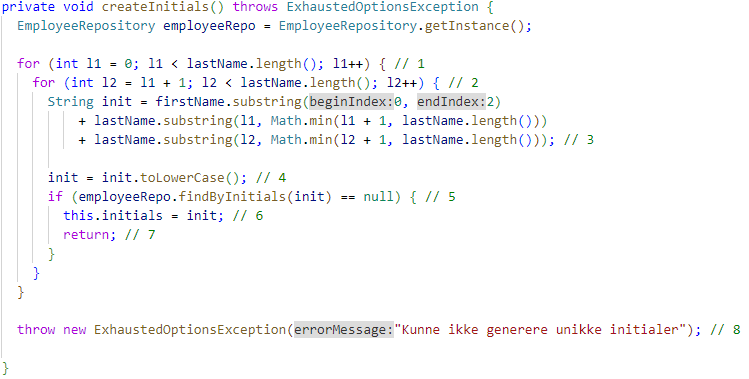
\includegraphics[width = \textwidth, keepaspectratio]{ImplementationAndTest/Diagrams/wb_create_initials.png}
    \label{fig:ep_create_initials}
\end{figure}
\noindent
For at gøre det bruger vi de execution paths, der er angivet i fig. \ref{fig:ep_create_initials} og skriver input-sæt, der sikrer, at alle execution paths dækkes.
\begin{table}[H]
\centering
\begin{tblr}{
  cells = {c},
  hline{1-2} = {-}{},
}
Execution path                                & Input set & Input property                                                                                 \\
1 (true), 2 (true), 3, 4, 5 (true), 6, 7         & A         & {There are fewer than 18 employees registered with\\first name "Michael", last name "Laudrup"} \\
1 (true), 2 (true), 3, 4, 5 (false), 8 & B         & {There are exactly 18 employees registered with first name\\~"Michael", last name "Laudrup"}   \\
1 (true), 2 (false), 8                 & C         & {There are exactly five employees registered with \\first name "Michael", last name "Laudrup"}   \\
1 (false), 8                              & B         & {There are exactly 18 employees registered with\\first name "Michael", last name "Laudrup"}    
\end{tblr}
\end{table}

\begin{table}[H]
\centering
\begin{tblr}{
  cells = {c},
  hline{1-2} = {-}{},
}
Input set & Input Data                                                                                  & Expected result                                                                                     \\
A         & {The employee repository is empty, \\and 18 employees named Michael Laudrup\\~are added.}   & {Initials are generated according to the description \\in the comment above createInitials.}        \\
B         & {The employee repository has 18 employees named\\~Michael Laudrup, and another is created.} & {An ExhaustedOptionsException is thrown with \\the message "Kunne ikke generere unikke initialer".}  \\
C         & {The employee repository has five employees named\\~Michael Laudrup, and another is created.} & {The sixth Michael Laudrup gets the initials miau} 
\end{tblr}
\end{table}
\subsection{generateProjectNumber()} 
\begin{figure}[H]
    \centering
    \caption{Execution paths i generateProjectNumber()}
    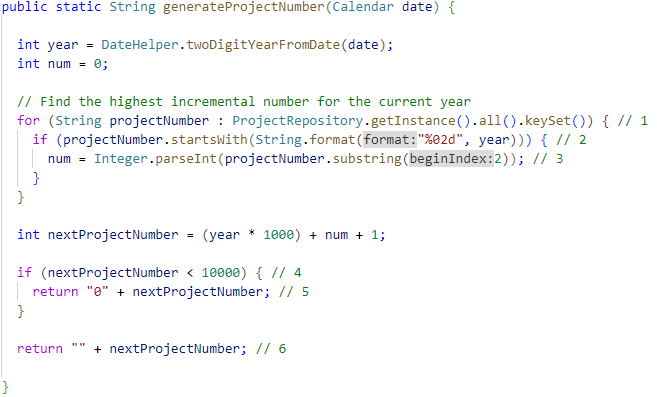
\includegraphics[width = \textwidth, keepaspectratio]{ImplementationAndTest/Diagrams/wb_genProjNum.png}
    \label{fig:ep_generate_project_number}
\end{figure}
\begin{table}[H]
\centering
\begin{tblr}{
  cells = {c},
  hline{1-2} = {-}{},
}
Execution path                                                     & Input set & Input property                                                                                                                  \\
{1 (not empty), 2 (true), 3, 4 (true), 5, 6} & A         & {There are projects from the current year, and the\\final two digits of the current year are \\less than 10}                    \\
{1 (not empty), 2 (true), 3, 4 (false), 6}   & B         & {There are projects from the current year, and the\\final two digits of the current year are\\greater than 10}                  \\
{1 (not empty), 2 (false), 4 (true), 5, 6}         & C         & {There is a project from a different year than the \\current, and the final two digits of the current\\year are less than 10}   \\
{1 (not empty), 2 (false), 4 (false), 6}           & D         & {There is a project from a different year than the\\current, and the final two digits of the current\\year are greater than 10} \\
1 (empty), 4 (true), 5, 6                                       & E         & {There are no projects and the final two digits of the\\~current year are less than 10}                                         \\
1 (empty), 4 (false), 6                                          & F         & {There are no projects and the final two digits of the\\current year are greater than 10}                                       
\end{tblr}
\end{table}                

\begin{table}[H]
\centering
\begin{tblr}{
  cells = {c},
  hline{1-2} = {-}{},
}
Input set & Input data                                                                                                      & Expected result                             \\
A         & {The current year is 2002 and there are two projects from the \\same year with project numbers 02001 and 02002} & {A new project with project number\\~02003} \\
B         & {The current year is 2023 and there are two projects from the \\same year with project numbers 23001 and 23002} & {A new project with project number\\~23003} \\
C         & {The current year is 2001 and there is a project from 2022 \\with project number 22001}                         & {A new project with project number\\~01001} \\
D         & {The current year is 2023 and there is a project from 2022\\with project number 22001}                          & {A new project with project number\\~23001} \\
E         & The current year is 2001 and there are no projects                                                              & {A new project with project number\\~01001} \\
F         & The current year is 2023 and there are no projects                                                              & {A new project with project number\\~23001} 
\end{tblr}
\end{table}

\subsection{createProjectActivity() \label{chap:white_box_create_project_activity}} 
Der kan oprettes projektaktiviteter for et projekt objekt. For at oprette en projektaktivitet, kræves at en medarbejder er logget ind og der skal bruges en titel, start- og slutuge. Derudover er det kun projektledere der kan oprette aktiviteter, hvis der er tildelt en projektleder til projektet. Herunder i \ref{lst:create_project_activity_source} er et udsnit af Project.java, inklusiv metoden der laves white box test for. White box testen udføres i praksis med JUnit, med filen CreateProjectActivityTest.java.


\begin{listing}[H]
    \centering
    \caption{createProjectActivity() source code}\label{lst:create_project_activity_source}
    \begin{minted}[breaklines]{java}
public class Project implements ConvertibleToViewModelInterface {

  private Employee projectLeader;
  private List<ProjectActivity> activities = new ArrayList<ProjectActivity>();

  public ProjectActivity createProjectActivity(String title, String startWeek, String endWeek, Employee loggedInUser)
      throws AlreadyExistsException, OperationNotAllowedException, InvalidPropertyException {
        
    if (hasProjectLeader()) { //1
      if (!projectLeader.isSameAs(loggedInUser)) { //2
        throw new OperationNotAllowedException("Kun projektlederen kan oprette en projekt aktivitet for dette projekt"); //3
      }
    }
    
    if (hasProjectActivity(title)) { //4
      throw new AlreadyExistsException("Projekt aktivitet findes allerede"); //5
    }
    
    ProjectActivity activity = new ProjectActivity(title, startWeek, endWeek); //6
    this.activities.add(activity); //7

    return activity;
  }
  
}

    \end{minted}
\end{listing}
% This centering command centers everything from here and down
%\centering
\begin{table}[H]

\caption{Execution paths in createProjectActivity()}\label{tbl:create_project_activity_paths}
\begin{tblr}{
  cells = {l},
  hline{1-2} = {-}{},
}
Execution path & 
Input set & 
Input property \\

{1 (false), 4 (false), 6, 7} & A & 
{
    \texttt{projectLeader} is null, \\ 
    \texttt{activities} does not contain an activity with title \texttt{title}
} \\

{1 (false), 4 (true), 5} & B & 
{
    \texttt{projectLeader} is null, \\ 
    \texttt{activities} contains an activity with title \texttt{title}
} \\

{1 (true), 2 (false), 4 (false), 6, 7} & C & 
{
    \texttt{projectLeader} is the same object as \texttt{loggedInUser},\\ 
    \texttt{activities} does not contain an activity with title \texttt{title}
} \\

{1 (true), 2(false), 4 (true), 5} & D & 
{
    \texttt{projectLeader} is the same object as \texttt{loggedInUser}, \\ 
    \texttt{activities} contains an activity with title \texttt{title}
} \\

{1 (true), 2(true), 3} & E & 
{
    \texttt{projectLeader} is another employee object than \texttt{loggedInUser}, \\
    \texttt{activities} does not contain an activity with title \texttt{title}
}\\

\end{tblr}
\end{table}                

\begin{table}[H]
\centering
\caption{Input sets for createProjectActivity()}\label{tbl:create_project_activity_inputs}
\begin{tblr}{
  cells = {l},
  hline{1-2} = {-}{},
}
Input set & 
Input data & 
Expected result \\

A & 
{
    \texttt{projectLeader} is null \\
    \texttt{activities} is empty \\
    \texttt{title} = "Planlægning" \\
    \texttt{startWeek} = "2101" \\ 
    \texttt{endWeek} = "2103" \\
    \texttt{loggedInUser} = \{"mila"\}
} & 
{
    \texttt{activities} contains a project activity \\ 
    with \texttt{title} "Planlægning"
} \\

B & 
{
    \texttt{projectLeader} is null \\
    \texttt{activities} = ["Planlægning"] \\
    \texttt{title} = "Planlægning" \\
    \texttt{startWeek} = "2101" \\ 
    \texttt{endWeek} = "2103" \\
    \texttt{loggedInUser} = \{"mila"\}
} & 
{
    Exception with message \\ 
    "Projekt aktivitet findes allerede" is thrown
} \\

C & 
{
    \texttt{projectLeader} = \{"mila"\} \\
    \texttt{activities} is empty \\
    \texttt{title} = "Planlægning" \\
    \texttt{startWeek} = "2101" \\ 
    \texttt{endWeek} = "2103" \\
    \texttt{loggedInUser} = \{"mila"\}
} & 
{
    \texttt{activities} contains a project activity \\ 
    with \texttt{title} "Planlægning"
} \\

D & 
{
    \texttt{projectLeader} = \{"mila"\} \\
    \texttt{activities} = ["Planlægning"] \\
    \texttt{title} = "Planlægning" \\
    \texttt{startWeek} = "2101" \\ 
    \texttt{endWeek} = "2103" \\
    \texttt{loggedInUser} = \{"mila"\}
} & 
{
    Exception with message \\ 
    "Projekt aktivitet findes allerede" is thrown
} \\

E & 
{
    \texttt{projectLeader} = \{"brla"\} \\
    \texttt{activities} is empty \\
    \texttt{title} = "Planlægning" \\
    \texttt{startWeek} = "2101" \\ 
    \texttt{endWeek} = "2103" \\
    \texttt{loggedInUser} = \{"mila"\}
} & 
{
    Exception with message \\ 
    "Kun projektlederen kan oprette en projekt aktivitet for dette projekt" is thrown
} \\

\end{tblr}
\end{table}

\subsection{findWorkTimeRegistrationById()}

For et givet projekt kan der oprettes projektaktiviteter, hvor en medarbejder kan angive mængden af arbejdstid han/hun har brugt på den pågældende aktivitet. Disse registreringer af arbejdstid bliver gemt med et id-nummer, som består af de positive naturlige tal og løber fra 1 og op. Dermed er det muligt at finde specifikke registreringer ud fra id-nummeret, og hertil benyttes metoden \texttt{findWorkTimeRegistrationById()}. 

Såfremt at id nummeret man søger efter, matcher det af en arbejdstidsregistrering, returneres den pågældende registrering. Hvis ikke der er et match, kastes en NotFoundException. Dette tester vi.

\begin{listing}[H]
    \centering
    \caption{findWorktimeRegistrationById() kildekode}\label{lst:find_work_time_registration_by_id_source_code}
    \begin{minted}[breaklines]{java}
public WorktimeRegistration findWorktimeRegistrationById(int id) throws NotFoundException {
    
    List<WorktimeRegistration> list = allWorktimeRegistrations(); // 1

    for (WorktimeRegistration worktimeRegistration : list) { // 2
        if (worktimeRegistration.getId().equals(id)) { // 3
            
            return worktimeRegistration; // 4
        }
    }

    throw new NotFoundException("Ukendt tidsregistrering"); // 5

}
    \end{minted}
\end{listing}

\begin{table}[H]
\centering
\caption{Execution paths i findWorktimeRegistrationById()}\label{tbl:find_worktime_registrations_by_id:execution_path}
\begin{tblr}{
  cells = {l},
  hline{1-2} = {-}{},
}
Execution path & 
Input set & 
Input property \\

{1 (empty), 2 (empty), 5} & A & 
{
    List containing work time registrations is empty, \\ 
    Arbitrary id number is set: \texttt{id} $=$ $1$
} \\

{1 (not empty), 2 (not empty), 3 (false), 5} & B & 
{
    List containing work time registrations has 1 element, \\ 
    Input id does not match a work time registration id
} \\

{1 (not empty), 2 (not empty), 3 (true), 4} & C & 
{
    List containing work time registrations has 5 elements,\\ 
    Input id matches a work time registration id
}

\end{tblr}
\end{table}  

\begin{table}[H]
\centering
\caption{Input sæt for findWorktimeRegistraionById()}\label{tbl:find_worktime_registrations_by_id:execution_path:inputs}
\begin{tblr}{
  cells = {l},
  hline{1-2} = {-}{},
}
Input set & 
Input data & 
Expected result \\

A & 
{
    \texttt{loggedInUser} = \{"mila"\} \\
    \texttt{id} = 1 \\
    \texttt{list} is empty \\
    
} & 
{
    Exception with message \\ 
    "Ukendt tidsregistrering" is thrown
} \\

B & 
{
    title of project activity = "Test" \\
    \texttt{loggedInUser} = \{"mila"\} \\
    "mila"\; registers work time = 5.0 \\
    \texttt{id} = 2 \\
    \texttt{list} has 1 element \\
} & 
{
    Exception with message \\ 
    "Ukendt tidsregistrering" is thrown
} \\

C & 
{
    title of project activity = "Test" \\
    \texttt{loggedInUser} = \{"mila"\} \\
    "mila"\; registers work time = 5.0 \\
    "mila"\; registers work time = 2.5 \\
    "mila"\; registers work time = 4 \\
    "mila"\; registers work time = 12.5 \\
    "mila"\; registers work time = 20 \\
    \texttt{id} = 4 \\
    \texttt{list} has 5 element \\
} & 
{
    \texttt{list} contains work time registration with matching id \\ 
    \texttt{worktimeRegistration} with work time = 12.5 is returned
} 
\end{tblr}
\end{table}

% !TeX root = ..\rapport_13_2.tex
\section{Code coverage}
\begin{figure}[H]
    \centering
    \caption{Coverage}
    
\includegraphics{ImplementationAndTest/Diagrams/jacoco.png}
    \label{fig:coverage}
\end{figure}
Nuff said
% !TeX root = ..\rapport_13_2.tex
\section{Design by contract}\label{chap:design_by_contract}

\subsection{generateProjectNumber} \label{sec:contract_generate_project_number}
pre: 
\begin{align}
    date \neq null
\end{align}
post:
\begin{align}
    \text{result } = \{s|\exists p \in projectRepository.getProjectNumbers : s \in p \land p = previousLargestProjectNumber + 1\}
\end{align}
\begin{align}
    3 + 4 = 7
\end{align}
\newline
\noindent
Med asserts ser det ud som følger:

\begin{listing}[H]
    \centering
    \caption{generateProjectNumber() med assertions}\label{lst:cgenerate_project_number_assertions}
    \begin{minted}[breaklines]{java}
public static String generateProjectNumber(Calendar date) {
  assert date != null // pre
  int year = DateHelper.twoDigitYearFromDate(date);
  int num = 0;

  // Find the highest incremental number for the current year
  for (String projectNumber : ProjectRepository.getInstance().all().keySet()) {
    if (projectNumber.startsWith(String.format("%02d", year))) {
      num = Integer.parseInt(projectNumber.substring(2));
    }
  }

  int previousProjectNumber = (year * 100) + num;
  int nextProjectNumber = (year * 1000) + num + 1;
  assert nextProjectNumber == previousProjectNumber + 1; // post
  
  if (nextProjectNumber < 10000) {
      return "0" + nextProjectNumber;
  }

  return "" + nextProjectNumber;

}
    \end{minted}
\end{listing}
\noindent
I virkeligheden er der to postconditions, i tilfælde af at preconditionen holder, sættes Employee-instancens initials-felt til init, i tilfælde af at den overtrædes, kastes en ExhaustedOptionsException.\\[4mm]
\subsection{createInitials()} \label{sec:contract_create_initials}
pre:
\begin{equation}
    nEmployeesWithName(employee) < maxInitials(employee)
\end{equation}
post:
\begin{equation}
    \{s | \exists e \in employeeRepository : s \in e.getInitials()\}
\end{equation}
Hvor maxInitials(employee) er $n$ vælg 2, hvor $n$ er længden af efternavnet, og duplikater fjernes i generationen af kombinationer.
I "Laudrup" (længde 7, $7 \choose 2$=21) går "lu", "au", "up" igen to gange, hvorfor der fås 18 og ikke de forventede 21. Der forklarer hvorfor white-box testens input er konstrueret som det er.\\[4mm]
Med asserts ser det ud som følger

\begin{listing}[H]
    \centering
    \caption{createInitials() med assertions}\label{lst:create_initials_assertions}
    \begin{minted}[breaklines]{java}
private void createInitials() throws ExhaustedOptionsException {
    EmployeeRepository employeeRepo = EmployeeRepository.getInstance();
    assert true; // pre

    for (int l1 = 0; l1 < lastName.length(); l1++) {
      for (int l2 = l1 + 1; l2 < lastName.length(); l2++) {
        String init = firstName.substring(0, 2)
            + lastName.substring(l1, Math.min(l1 + 1, lastName.length()))
            + lastName.substring(l2, Math.min(l2 + 1, lastName.length()));

        init = init.toLowerCase();
        if (!employeeRepo.initialsExist(init)) {
          this.initials = init;
          assert this.initials == init; // post
          return;
        }
      }
    }

    throw new ExhaustedOptionsException("Kunne ikke generere unikke initialer");
  }
    \end{minted}
\end{listing}
\noindent
Implicit garanteres det der står i createInitials' precondition gennem funktionens kørsel, derfor assertes blot true som precondition. I virkeligheden er der to postconditions, i tilfælde af at preconditionen holder, sættes Employee-instancens initials-felt til init, i tilfælde af at den overtrædes, kastes en ExhaustedOptionsException.\\[4mm]

\subsection{createProjectActivity()} \label{sec:contract_create_project_activity}
pre: 
\begin{equation}
    title \neq null \wedge startWeek \neq null \wedge endWeek \neq null \wedge loggedInUser \neq null \wedge activities \neq null
\end{equation}

post: 
\begin{equation}
\begin{gathered}
    activity \in activities \wedge \\
    \neg project@pre.hasProjectActivity(title) \wedge \\
    (hasProjectLeader() \to projectLeader.isSameAs(loggedInUser))
\end{gathered}
\end{equation}

\begin{listing}[H]
    \centering
    \caption{createProjectActivity() kildekode med assertions}\label{lst:create_project_activity_assertions}
    \begin{minted}[breaklines]{java}
  public ProjectActivity createProjectActivity(String title, String startWeek, String endWeek, Employee loggedInUser)
      throws AlreadyExistsException, OperationNotAllowedException, InvalidPropertyException {

    assert title != null;
    assert startWeek != null;
    assert endWeek != null;
    assert loggedInUser != null;
    assert activities != null;

    if (hasProjectLeader()) {
      if (!projectLeader.isSameAs(loggedInUser)) {
        throw new OperationNotAllowedException("Kun projektlederen kan oprette en projekt aktivitet for dette projekt");
      }
    }

    if (hasProjectActivity(title)) {
      throw new AlreadyExistsException("Projekt aktivitet findes allerede");
    }

    ProjectActivity activity = new ProjectActivity(title, startWeek, endWeek);
    this.activities.add(activity);

    /**
     * NOTE: This post condition does not check for 
     * !project@pre.hasProjectActivity(title)
     */
    assert (
      activities.contains(activity) &&
      (!hasProjectLeader() || projectLeader.isSameAs(loggedInUser) )
    );

    return activity;
  }
    \end{minted}
\end{listing}


\subsection{findWorktimeRegistrationById()} \label{sec:contract_findd_work}
\noindent Precondition: I dette tilfælde er vores precondition \texttt{true}, da vores postconditions korrigerer for fejl, så alle tilfælde af inputs fejlhåndteres.

%\begin{align}
    %allWorktimeRegistrations().size()\; >\; 0 \;\wedge\; id \; \in %\; \mathbb{N} \; \wedge \; 0 \; < \; id  \; <=\; %allWorktimeRegistrations().size()
%\end{align}


\noindent
Postcondition: 
\begin{equation}
    \exists i\; :\; (result = i \iff\; \exists worktimeRegistration.getId() \; = \; i\; \lor result = NotFoundException)
\end{equation}\label{postcondition 1}

Det skal nævnes, at postconditionen, i tilfælde af at leddet før $\lor$ i ligningen over 


\begin{listing}[H]
    \centering
    \caption{findWorktimeRegistrationById() kildekode med assertions}\label{lst:find_work_time_registration_by_id_assertions}
    \begin{minted}[breaklines]{java}
public WorktimeRegistration findWorktimeRegistrationById(int id) throws NotFoundException {

    assert true // Precondition
    
    List<WorktimeRegistration> list = allWorktimeRegistrations();

    for (WorktimeRegistration worktimeRegistration : list) {
        if (worktimeRegistration.getId().equals(id)) {
            assert list.stream().anyMatch(x -> x.getId() == id) // Postcondition
            
            return worktimeRegistration;
        }
    }

    throw new NotFoundException("Ukendt tidsregistrering");

}
    \end{minted}
\end{listing}



% !TeX root = ..\rapport_13_2.tex
\section{Design mønstre} \label{chap:design}
Der har været fokus på at adskille præsentationslag, businesslag, og persistence-lag og flere design mønstre er anvendt for at opnå et let læseligt, overskueligt og lavt koblet system. 

\subsection{Program-lag}
Et fuldt klassediagram over program-laget kan ses i appendix \ref{apdx:classDiagram_full}. Et simplificeret klassediagram herunder i \ref{fig:class_persistency_layer} viser relationer mellem klasserne i TaskFusion programmet. TaskFusion fungere som hovedklasse og er primært ansvarlig for brugergodkendelser. Et facade mønster (eng: Facade pattern) er implementeret med \texttt{EmployeeFacade.java} og \texttt{ProjectFacade.java} for at opnå lav kobling. F.eks. bliver systemet, der behandler employees, tilgået gennem \texttt{EmployeeFacade.java} således at klasserne, bestående af bl.a. \texttt{EmployeeRepository.java}, \texttt{Employee.java}, \texttt{RegularActivity.java}, ikke skal kaldes af klienten på forskellig vis. I stedet kan klienten tilgå alle de nødvendige egenskaber igennem facaden kun. Sammen med \textit{EmployeeFacade} og \textit{ProjectFacade} eksponere \textit{TaskFusion} de offentlige metoder der skal kunne tilgås i programmet. På den måde kan vi frihed til at ændre alle metoder i de resterende program-lag, uden det vil påvirke eventuelle brugergrænseflader. Alle metoder i \textit{facade} klasserne kan i virkeligheden ligge i TaskFusion klassen, men ved at opdele metoderne i passende seperate klasser, kan vi bedre vedligeholde og udbygge programmet. 
Programmets domæne lag består af instantierbare objektklasser og er ansvarlig for \textit{Business-logic}. Persistency-laget indeholder \textit{Repositories}, der er ansvarlige for kommunikation med en lagringsløsning. Selvom programmet ikke har et database lag på nuværende tidspunkt, vil det være let at bygge flere lagringsløsninger på senere, ved kun at skulle modificere persistency klasserne. 

\begin{figure}[H]
    \centering
    \caption{Klassediagram over program-lag}
    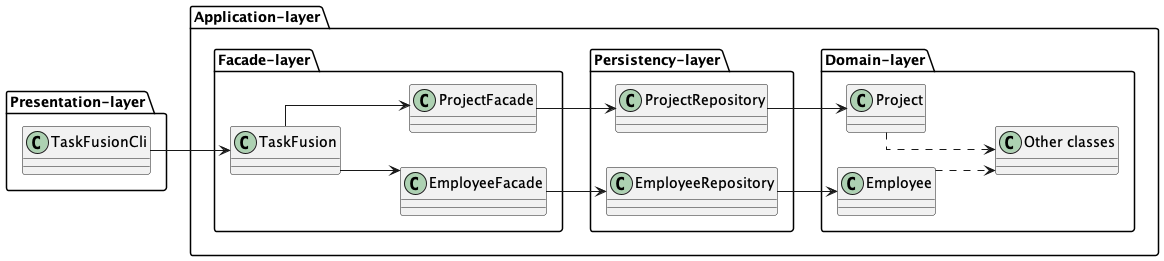
\includegraphics[width = \textwidth, keepaspectratio]{TaskFusion/out/assets/diagrams/class_persistency_layer/ClassDiagram_layer.png}
    \label{fig:class_persistency_layer}
\end{figure}

Vi ønsker desuden aldrig at eksponere programmets klasser udenfor program-laget. Derfor implementere alle instantierbare klasser i domæne-laget \textit{ConvertibleToViewModel}-interfacet, vist herunder i \ref{fig:class_persistency_domain}. Dette interface kræver at klasserne kan eksporteres til en tilsvarende visningsklasse til brug i præsentations-lag. På den måde kan vi undgå at brugere kan kalde metoder fra domæne-laget, og dermed sikre de forudsætninger de enkelte metoder måtte have.

\begin{figure}[H]
    \centering
    \caption{Domæne-laget}
    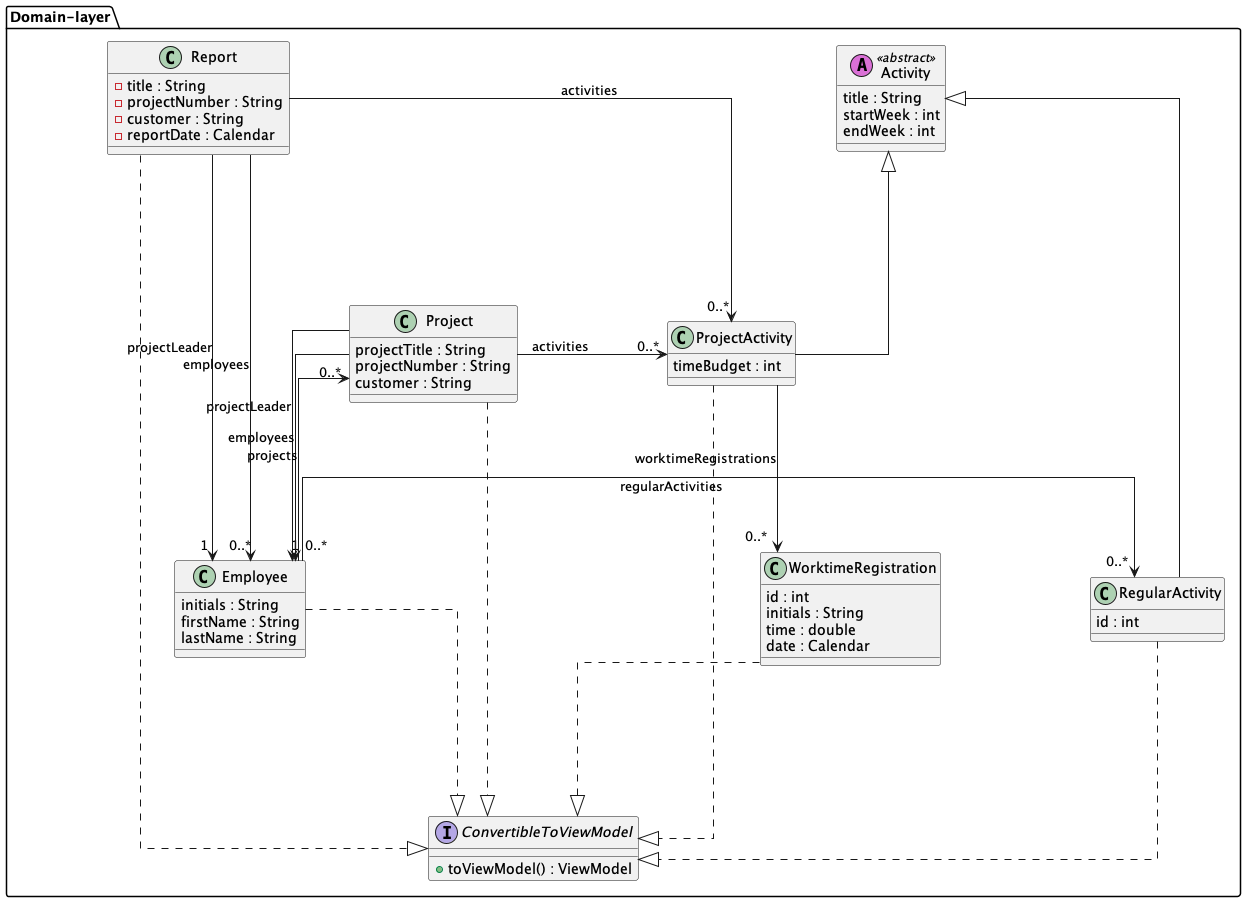
\includegraphics[width = \textwidth, keepaspectratio]{TaskFusion/out/assets/diagrams/class_persistency_domain/ClassDiagram_domain.png}
    \label{fig:class_persistency_domain}
\end{figure}

Et andet design mønster der er taget i brug, er singleton design mønstret. F.eks. haves et opbevaringssted for alle medarbejdere kaldet \textit{EmployeeRepository}. Der ønskes kun én instans af dette objekt, da idéen er at tilgå og opbevare medarbejderne via. ét objekt. Hvis flere instanser af dette objekt skulle forekomme, er det ikke sikret, at brugeren kan tilgå alle medarbejderne fra den ene instans, da medarbejdere kan eksistere i de andre instanser, hvorfor objektet skal være en singleton. Af samme grunde som EmployeeRepository er en singleton, er ProjectRepository ligeså.


\subsection{Præsentations-laget}
Som det blev nævnt i indledningen af dette kapitel, har der været fokus på adskillelse af de forskellige lag i arkitekturen af programmet. Måden hvorpå business-logikken er blevet separeret fra præsentationslaget i programmet er ved brug af Model-View-Controller design mønstret. Dette er gjort ved at have ’controller’ klasser og ’view’ klasser, som har funktionen at modtage forespørgsler fra brugeren og fremvise det efterspurgte data uden at have noget business logik i sig. Disse kan ses under mapperne \textit{controllers} og \textit{views}.

\subsubsection{CLI klassediagram}
\textit{TaskFusionCLI} er hovedklassen når TaskFusion programmet skal benyttes igennem en CLI brugergrænseflade. Når grænsefladen skal interagere med TaskFusion programmet, foregår al kommunikation imellem \textit{Facade}-laget. CLI'en er fundamentalt opbygget med tanke på genbrugelighed, og simplicitet. Det er opnået ved at tage udgangspunkt i en \textit{MenuController}, hvorfra \textit{View}'s bruges til at skrive information brugeren efterspørger til konsollen. Hvordan et \textit{View} ser ud for brugeren, afhænger af hvilke variabler og objekter der gives ved konstruktion af \textit{View}'et. \textit{Component}-klasser er en form for hjælpe klasser, der igennem \texttt{public static} metoder, tilbyder universelle komponenter til brug i grænsefladen.

\begin{figure}[H]
    \centering
    \caption{Klassediagram over præsentations-laget}
    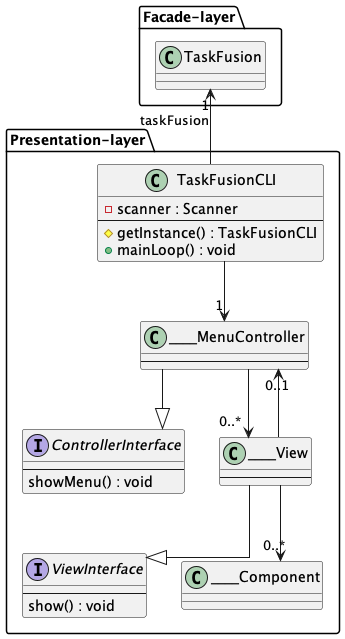
\includegraphics[width = 5cm, keepaspectratio]{TaskFusion/out/assets/diagrams/class_cli/TaskFusion-CLI.png}
    \label{fig:class_cli}
\end{figure}

\subsubsection{CLI brugergrænsefladen}
Da CLI grænsefladen til TaskFusion er opbygget af \textit{MenuController}'re og \textit{View}'s, ender vi da også med et netværk af mulige veje brugeren kan gå. For at få et overblik over TaskFusion, er herunder i \ref{fig:flow_cli} et \textit{flow}-diagram over menuer og sider i CLI grænsefladen. Diagrammet er ikke tiltænkt at være noteringsmæssig korrekt, men har fungeret effektivt som mockup i udviklgsfasen, og stadig til at skabe et overblik over programmet. En større version af figuren kan ses i appendix \ref{apdx:classDiagram_presentation}.
\begin{figure}[H]
    \centering
    \caption{Flowdiagram over CLI brugergrænsefladen}
    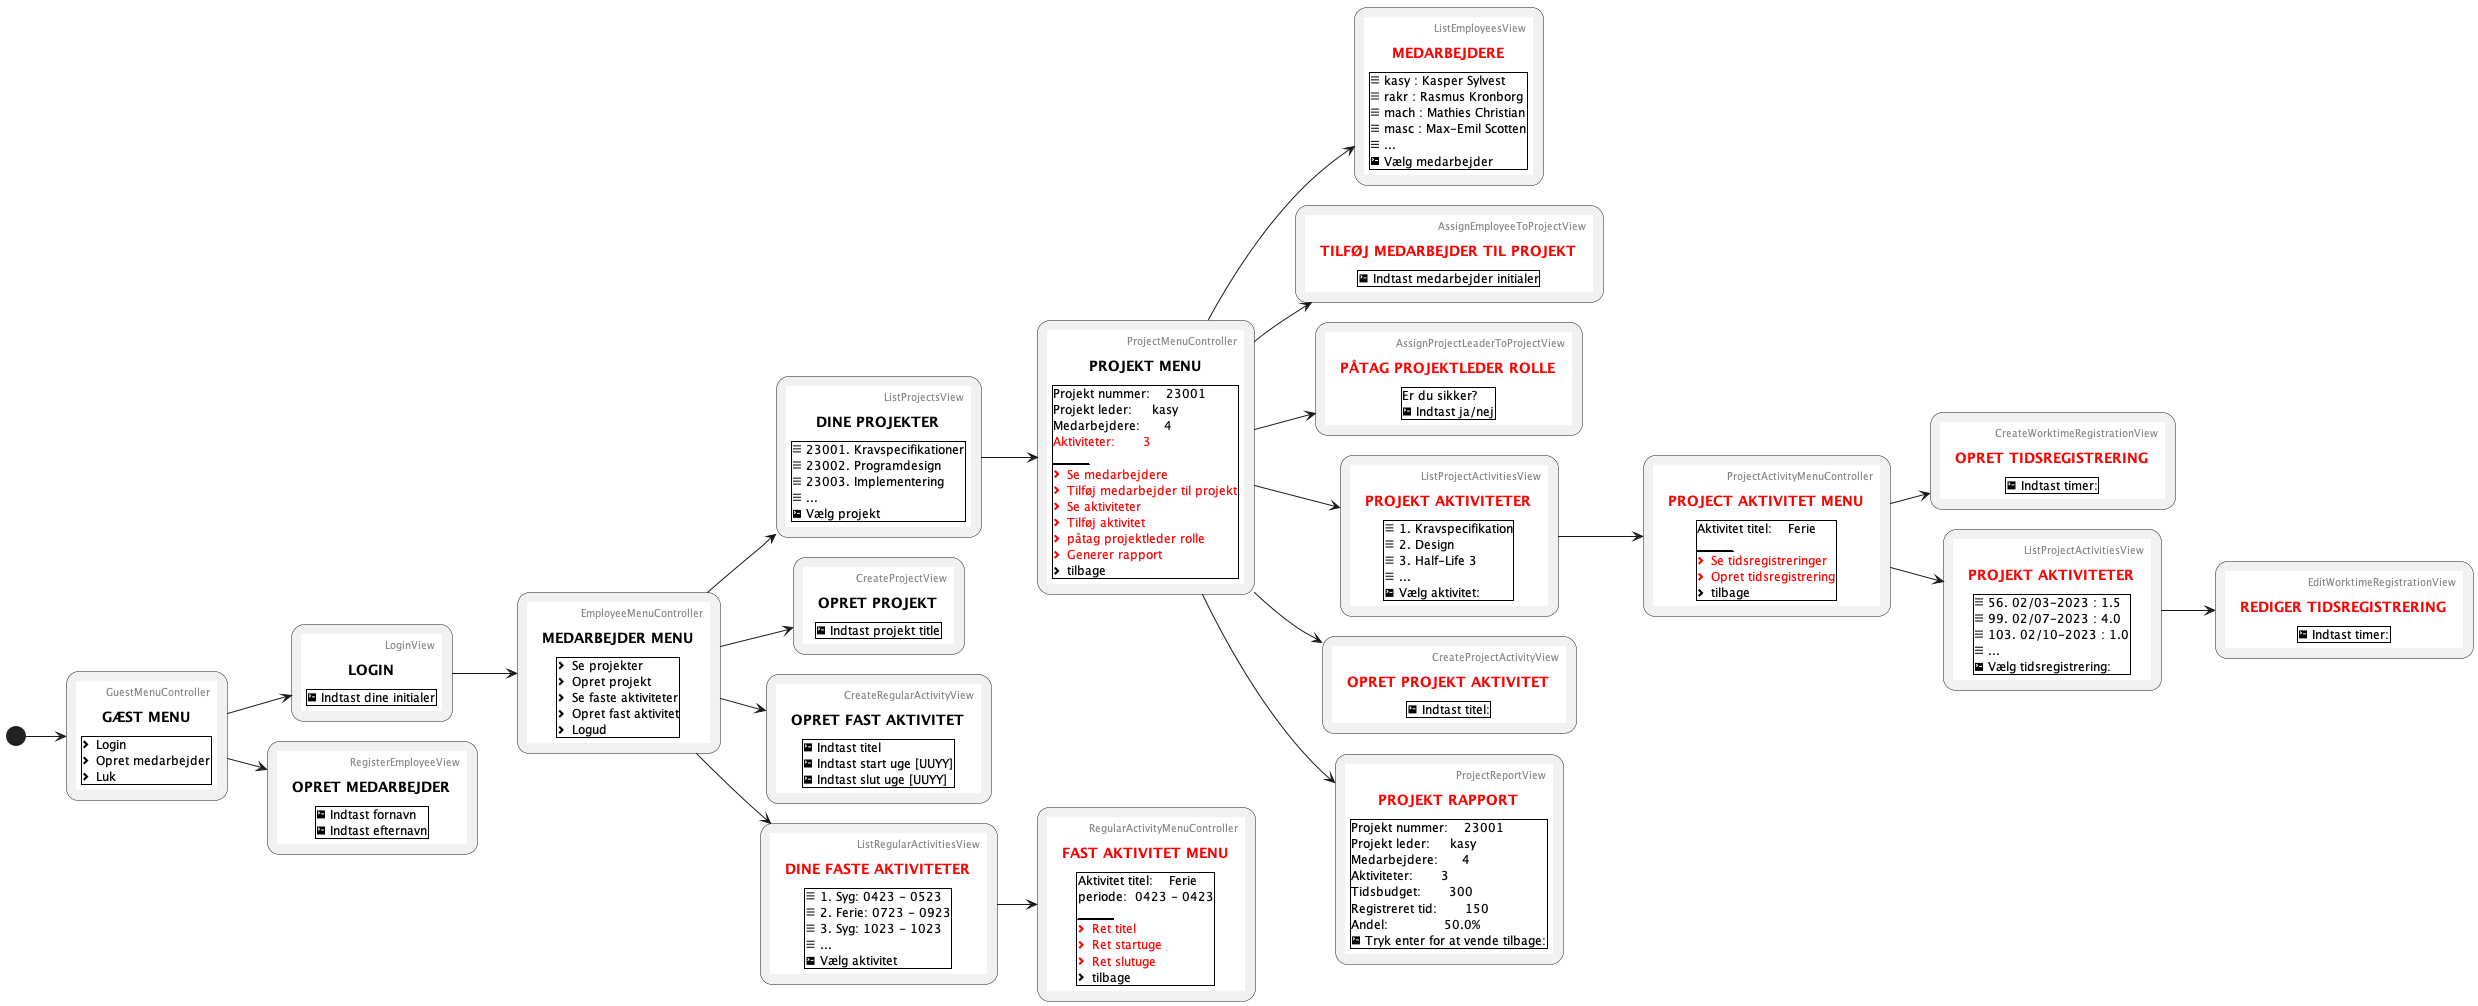
\includegraphics[width = 11cm, keepaspectratio]{TaskFusion/out/assets/diagrams/flow_cli/flow_cli.png}
    \label{fig:flow_cli}
\end{figure}
% !TeX root = ..\rapport_13_2.tex
\section{Konklusion}

%Bibliography herunder:
%\newpage

%\bibliographystyle{unsrtnat}
%\bibliography{Bibliography}

\newpage

\listoffigures
%\newpage
\listoftables
%\newpage
\listoflistings
%Appendicer herunder:
% !TeX root = ..\..\rapport_13_2.tex
\newpage
\appendix
\appendixpage
\addappheadtotoc
\section{Sekvensdiagram: CreateProjectActivity()}\label{apdx:seq_create_project_activity}
\begin{figure}[H]
    \centering
    \caption{Sekvensdiagram: Opret projektaktivitet}\label{fig:sequenceCreateProjectActivity}
    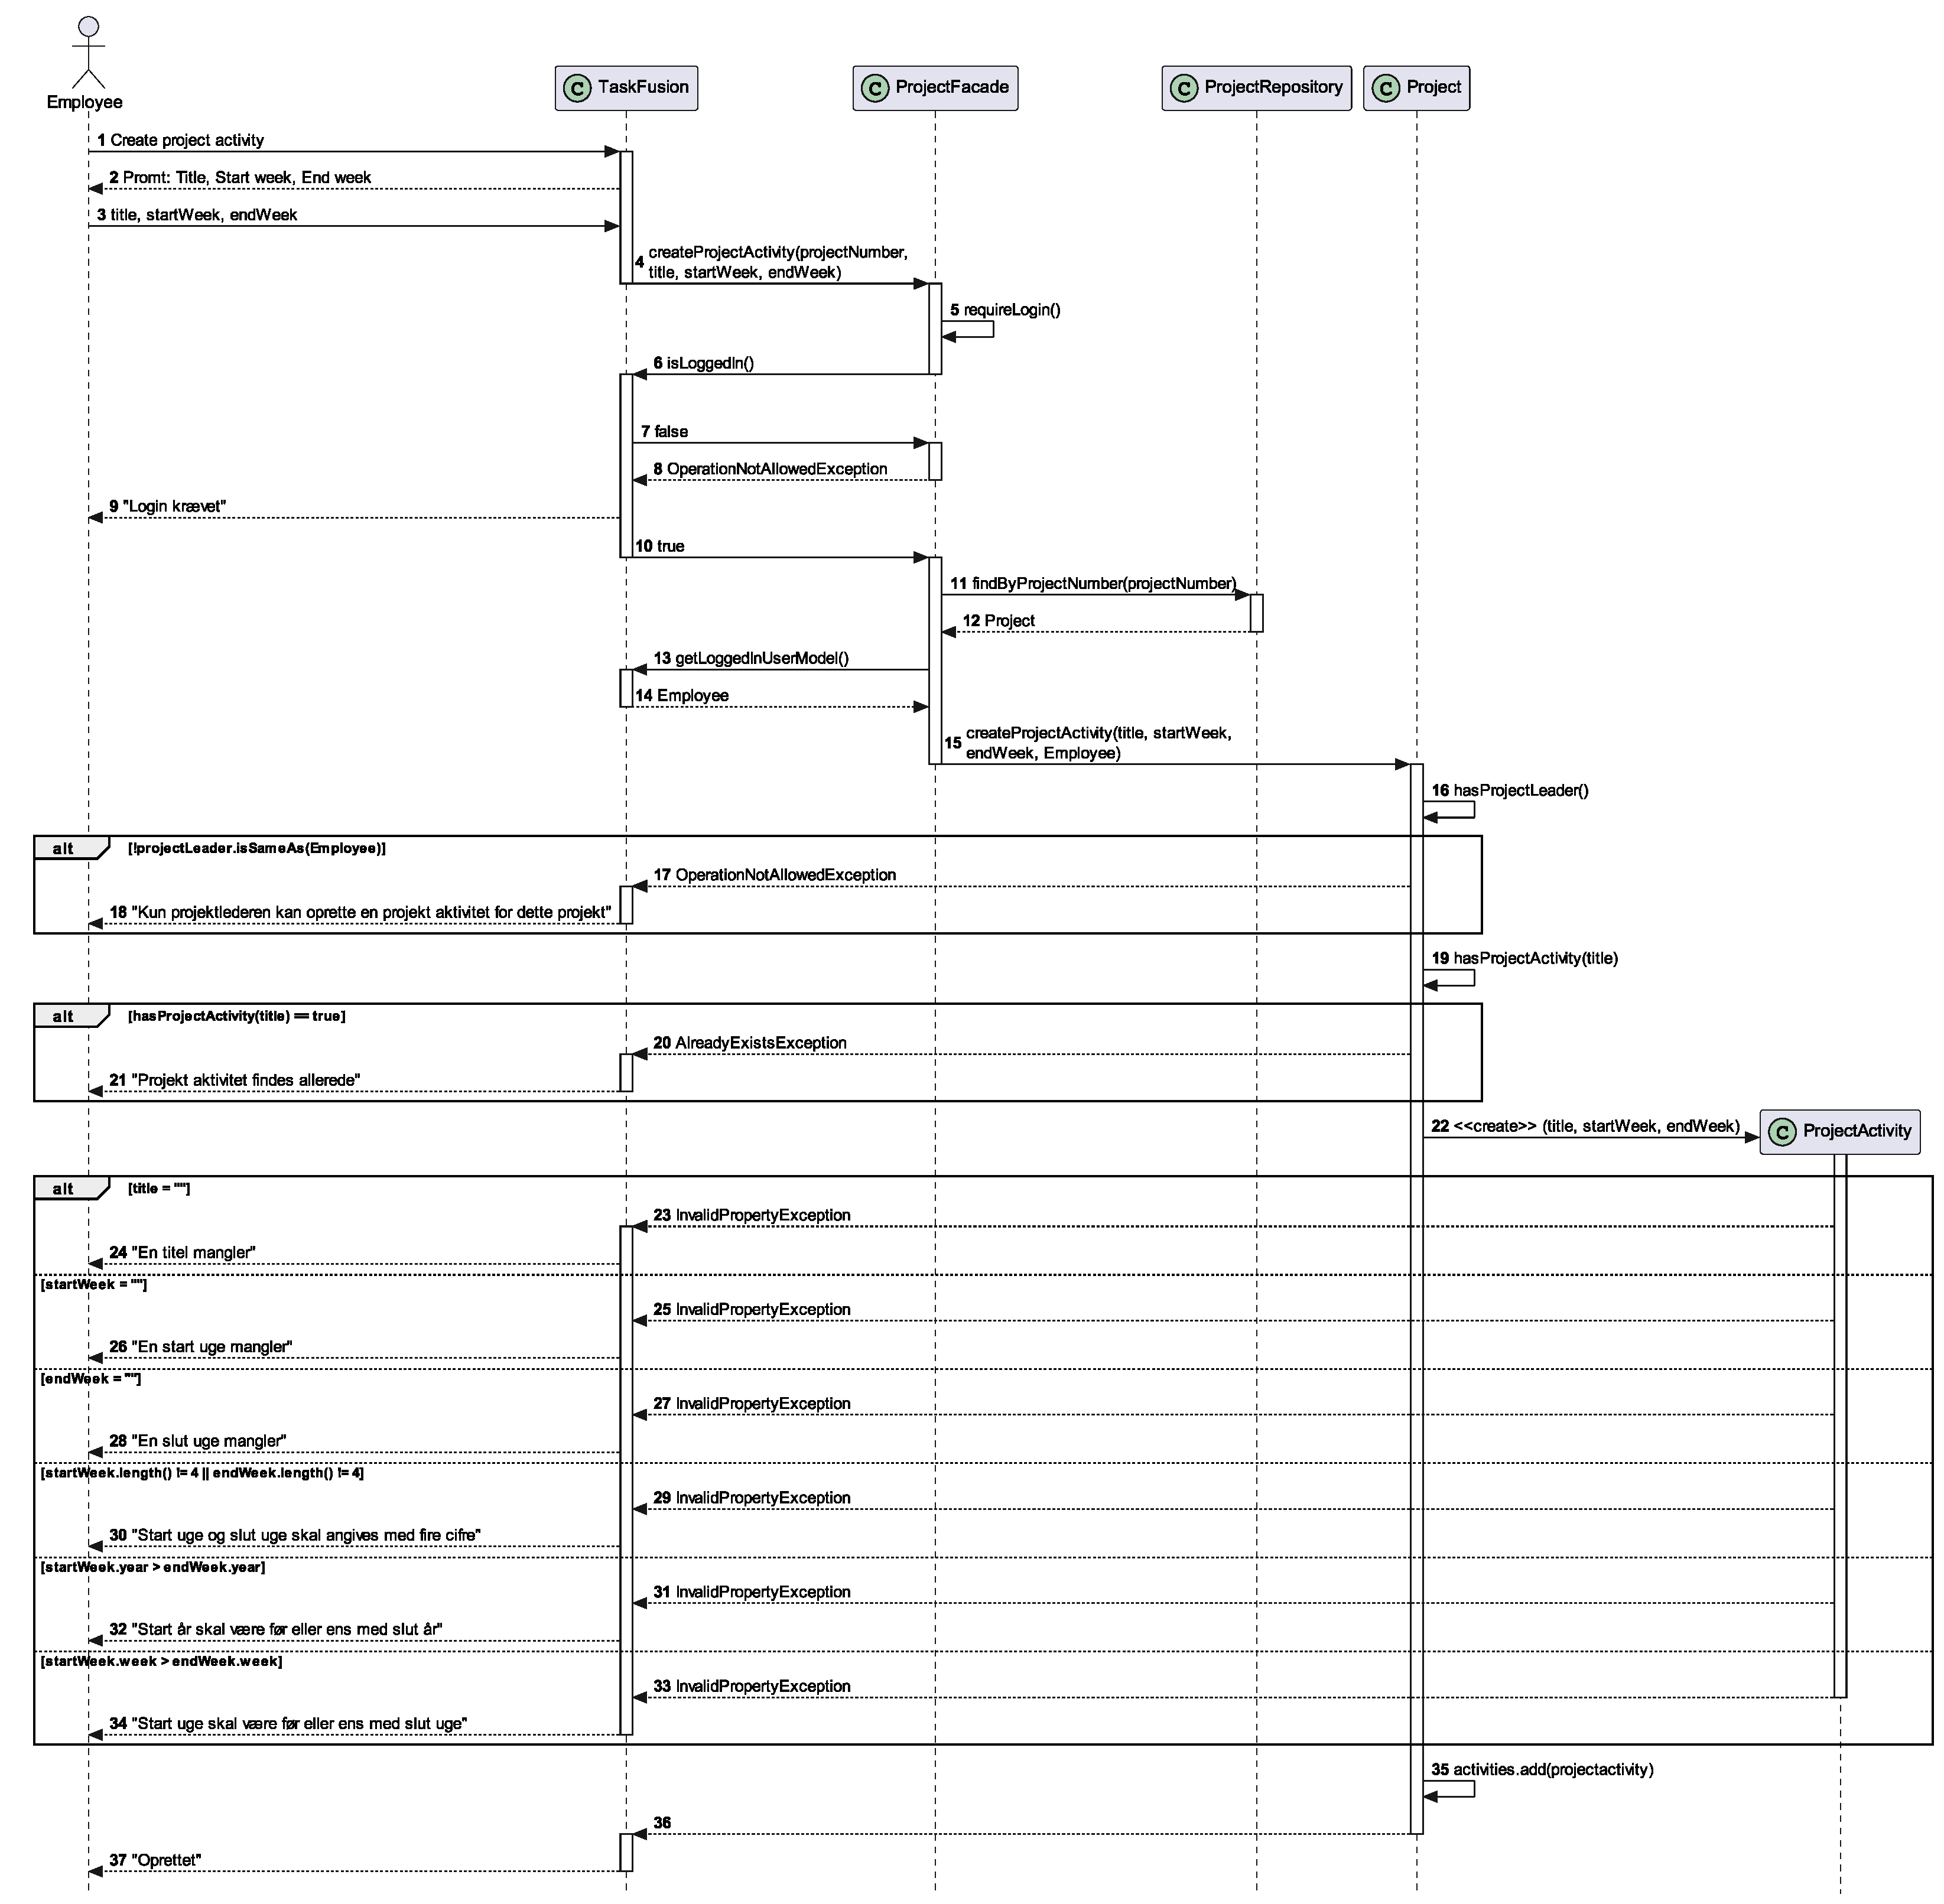
\includegraphics[width=.8\textwidth]{RequirementsAndDesign/SequenceDiagrams/seqCreateProjectActivity.eps}
\end{figure}
\begin{landscape}
    \section{Klassediagram over program laget}\label{apdx:classDiagram_full}
    \begin{figure}[H]
        \centering
        \caption{Klassediagram over program laget}
        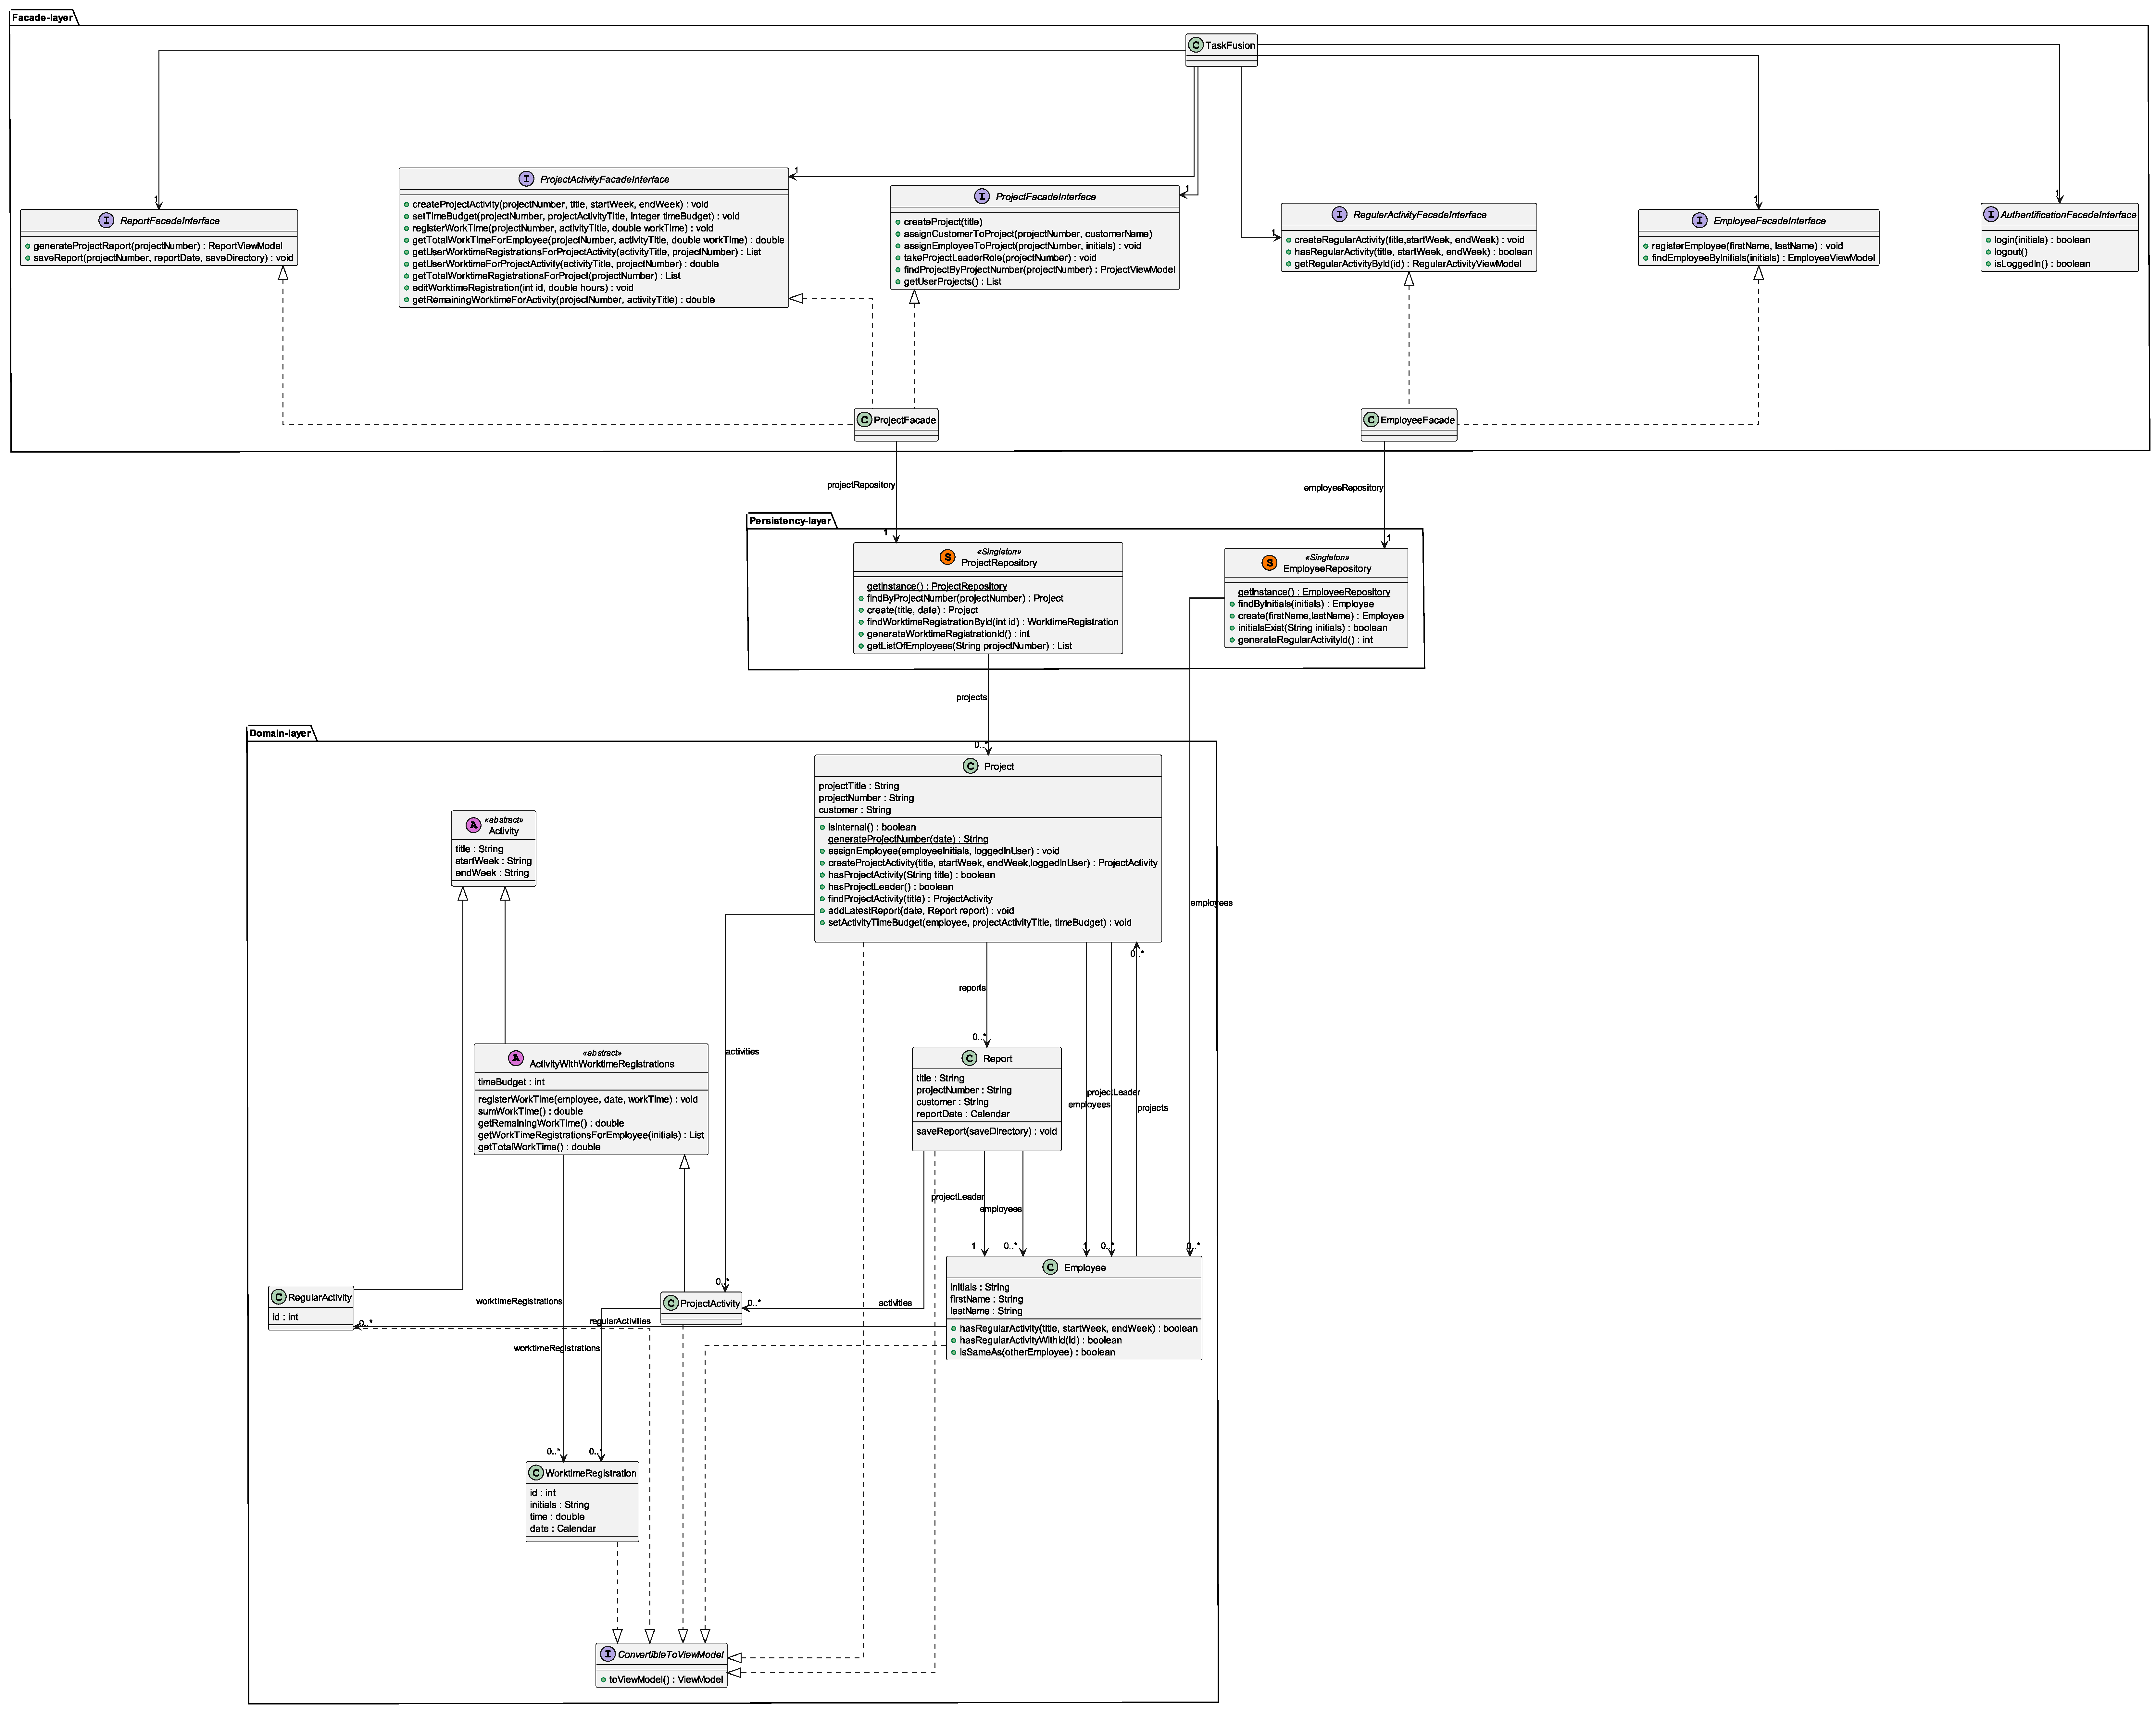
\includegraphics[width = \textheight]{ImplementationAndTest/Diagrams/ClassDiagrams/ClassDiagram_full.eps}
        \label{fig:classDiagram_full}
    \end{figure}
    \section{Klassediagram over præsentations-laget}\label{apdx:classDiagram_presentation}
    \begin{figure}[H]
        \centering
        \caption{Flowdiagram over CLI brugergrænsefladen}
        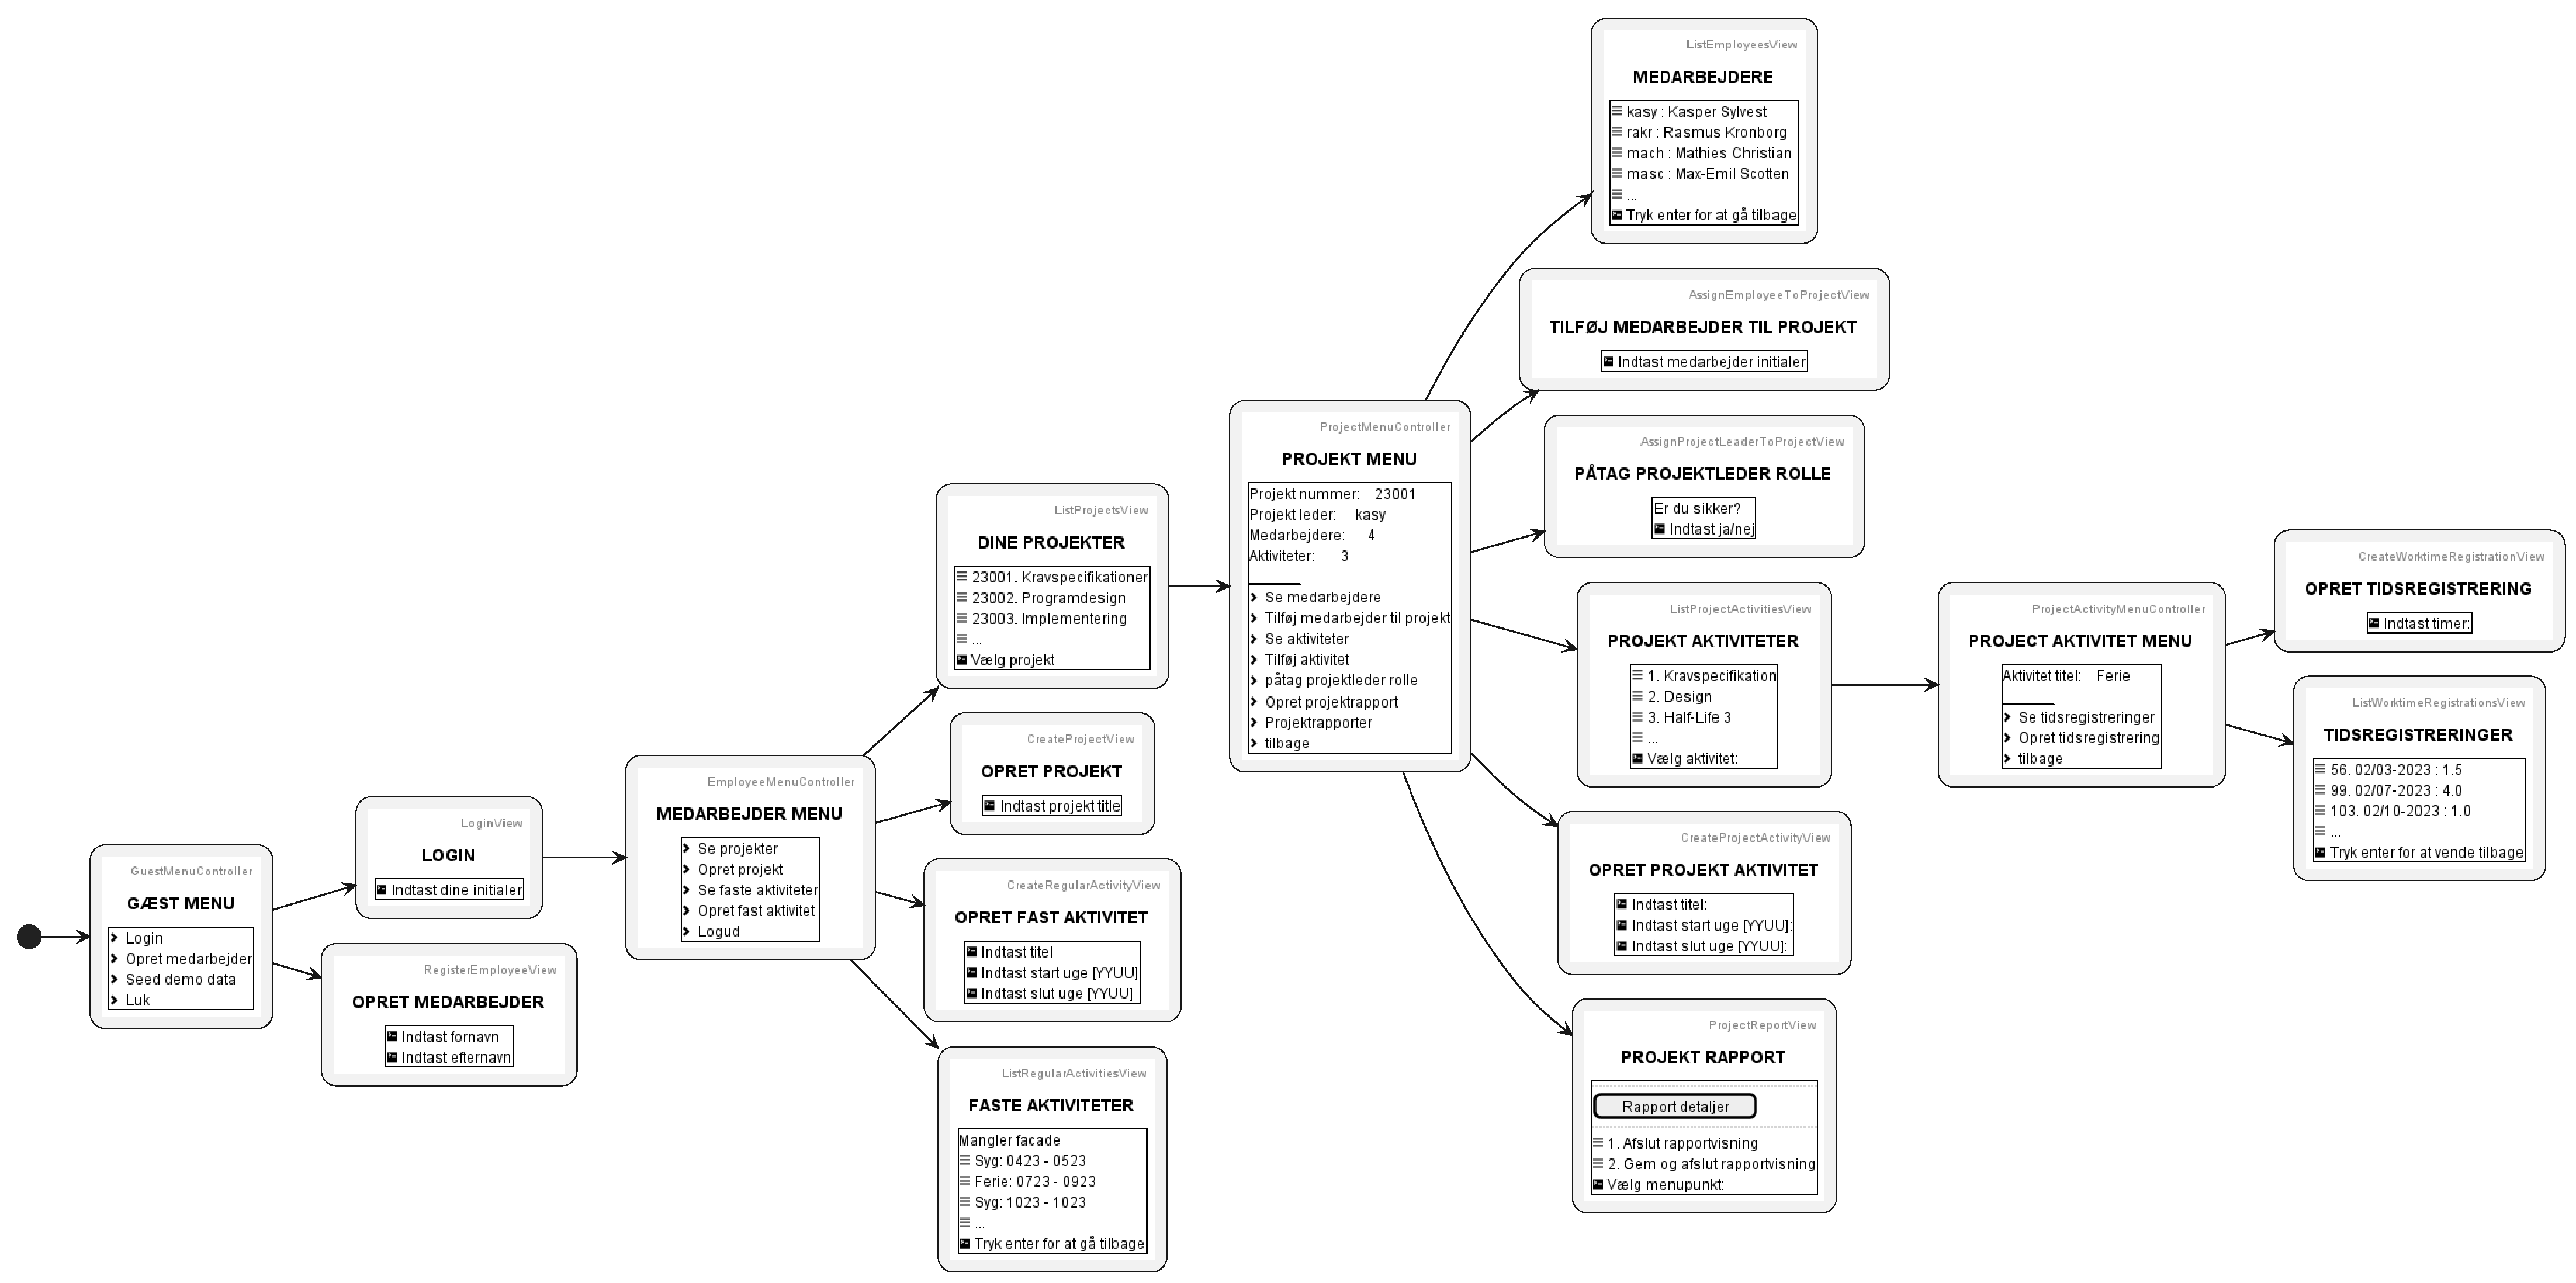
\includegraphics[width = \linewidth]{ImplementationAndTest/Diagrams/FlowCharts/flow_cli.eps}
        \label{fig:flow_cli_big}
    \end{figure}
    \section{Klassediagram over facade-laget}\label{apdx:classDiagram_facade_full}
    \begin{figure}[H]
        \centering
        \caption{Detaljeret klassediagram af facade-laget}
        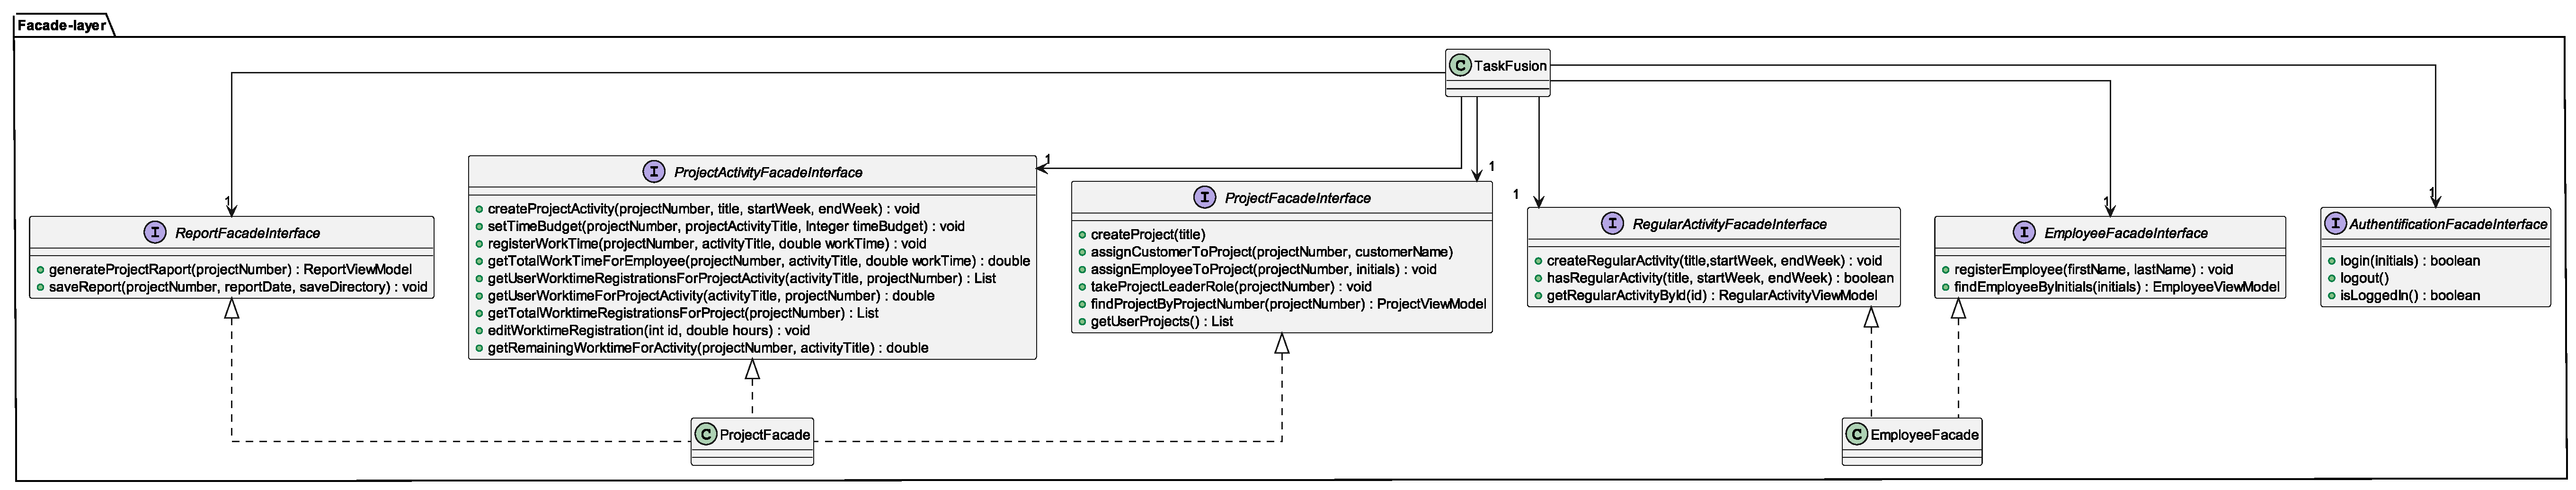
\includegraphics[width = \linewidth]{ImplementationAndTest/Diagrams/ClassDiagrams/ClassDiagram_facade_full.eps}
        \label{fig:class_facade_full}
    \end{figure}
\end{landscape}

\end{document}
